%!TEX root = ./icml2016.tex

\section{Related Work}

The literature on data factorisation and vector space models for 
relational data is vast. 
%or low-rank approximation is vast. 
We give a brief overview of related work along three design choices:
%with respect to three orthogonal dimensions, 
the method, the learning strategy, and the data representation. 
We then use these dimensions to help position our work. 
\begin{description}
%\item[Statistical method] With an statistical assumption used to develop 
%underlying model structure, we broadly categorise models into Bayesian 
%and non-Bayesian models.
\item[Bayesian/Non-Bayesian] This refers to two broad classes of model 
formulation, whether the obtained model is a point estimate or posterior 
distribution, whether to incorporate priors, quantification of uncertainty, 
and so on. 
%\item[Learning strategy] The models passively learn from labels of given 
%data points, or the models actively learn by  requesting data points 
%to be labeled.
\item[Passive/Active] This refers to two different learning strategies, 
of passively learning a model given labeled data points, or actively 
requesting data points to be labeled.
\item[Matrix/Tensor/Composition] Relational learning problems for operate on 
different data representations. Matrix representation is common when a dataset 
can be represented as a bi-partite graph, such as (user, item) tuples in the 
recommender systems setting. Tensor representation is handy when edges in the 
graph have labels, i.e. (entity1, relation, entity2). We can think of 
compositions as paths in the graph, i.e. entity1 -- relation1 -- entity2 -- 
relation2 -- entity3.
%\item[Data representation] Data for a factorisation problem can be 
%represented as a matrix or tensor. A graph representation of tensor reveals
%a compositional structure of the data.
\end{description}
In Table \ref{tbl:relatedwork}, we summarise a sample of related recent work 
along all combinations in each dimension. 
Note that N,A,C, or Non-Bayesian Active Composition model, can be done by 
simply using the query strategies from \citet{kajino2015active} on the 
compositional model by \citet{guu2015traversing}. Our work address a critical gap 
in Bayesian Tensor factorisation capable of learning in the 
Active setting with relation Compositions.
\eat{The knowledge base construction has been widely focused in the natural 
language processing communities. 
Manual data acquisition with human crafted 
or automatically inferred synthetic rules or distant supervision on a large
amount of unlabelled text are the main tools to construct \cite{fader2011identifying,Mintz2009}.}

Given this position, our work is inspired by, and most closely related to:
%Recently, 
active multi-relational data construction (AMDC) 
with tensor factorisation~\cite{kajino2015active}, 
Thomson sampling for matrix factorisation~\cite{kawale2015efficient}, 
and compositions objectives in vector space~\cite{guu2015traversing}.
Note that we re-formulate the compositions objectives probabilistically such that it can be used in an active setting; 
our approach for active learning is a generalisation of
Thomson sampling from matrixes to tensors; 
AMDC find that reconstruction accuracy and recall 
cannot be achieved at the same time with strategies geared towards 
either exploit or reducing uncertainty, 
we show that the two objectives can be achieved at the same time with 
a properly designed exploration and exploitation scheme. 

\eat{show active knowledge base construction
algorithm based on the low-rank structure. They proposed active 
multi-relational data construction (AMDC) with two separate problems: 
a knowledge base population and predictive model construction, and show 
that these two goals cannot be achieved at the same time. In this work, 
we show that it can be achieved at the same time with a properly designed
exploration and exploitation scheme that has been shown in the matrix 
factorisation problem \cite{kawale2015efficient}.
}


%\begin{itemize}
%\item [B,A,M] Efficient Thompson Sampling for OnlineMatrix-Factorization Recommendation\cite{kawale2015efficient}. Active learning and search on low-rank matrices \cite{sutherland2013active}. Collaborative filtering as multi armed bandit \cite{guillou2015collaborative}
%\item [N,A,M] Matrix completion with queries \cite{ruchansky2015matrix}.
%\item [B,P,M] PMF \cite{mnih2007probabilistic} ...
%\item [N,P,M] NMF\cite{lee1999learning} ...
%\item [B,P,T] Bayesian Tensor Factorisation models. CANDECOMP/PARAFAC (CP) decomposition \cite{xiong2010temporal,schmidt2009probabilistic}, CP and TUCKER3 \cite{yilmaz2012algorithms}
%\item [N,A,T] Populating knowledge graph with active learning (IBM) \cite{kajino2015active}
%\item [N,P,T] Rescal \cite{nickel2011three}, TransE \cite{bordes2013translating}, and many others.
%\item [N,P,C] Compositional vector space model \cite{Neelakantan2015}, 
%\end{itemize}
%
%Might be relevant, but not positioned in the figure.
%\begin{itemize}
%\item Clustering based Bayesian approach for learning relations: Infinite relational model based on entity clustering \cite{kemp2006learning}.
%\item Path ranking algorithm (graph feature model) \cite{Lao2010}
%\end{itemize}

%\begin{figure}[t]
%	\centering
%	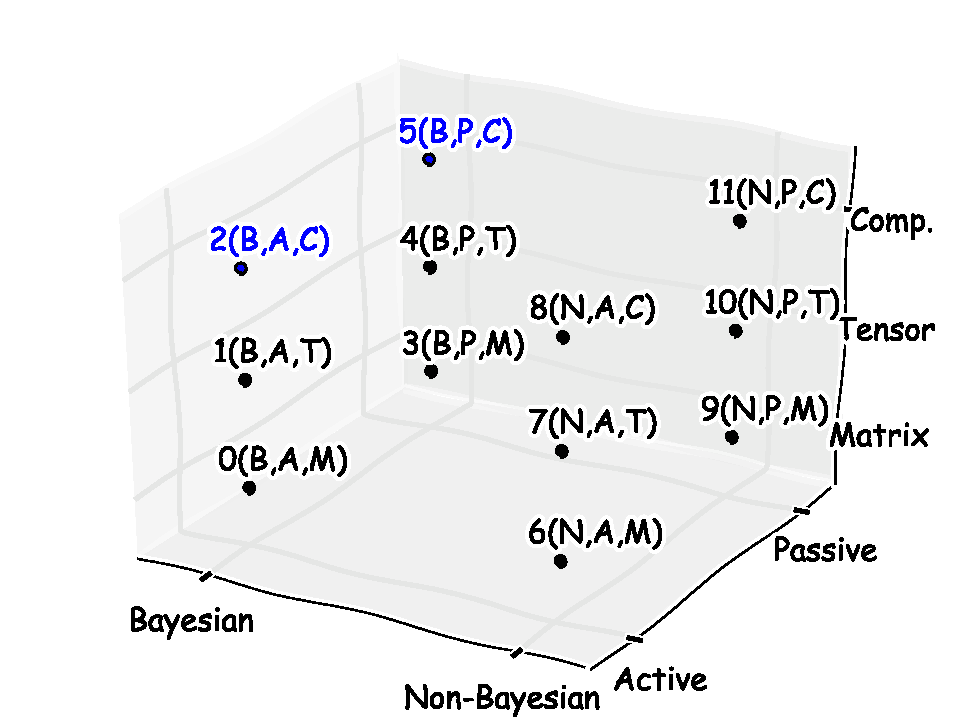
\includegraphics[width=\linewidth]{images/3d_plot.pdf}			
%	\caption{\label{fig:related3d}Scope of our work}
%\end{figure}
